\documentclass{article}

\usepackage{graphicx}
\usepackage{fancyhdr}
\usepackage[sorting=none]{biblatex}
\usepackage[margin=1in]{geometry}
\usepackage{listings}
\usepackage[hidelinks]{hyperref}
\usepackage{xcolor}
\usepackage{xepersian}
\usepackage{ltablex}
\usepackage{booktabs, makecell, longtable}



\addbibresource{bibliography.bib}
\settextfont[Scale=1.2]{IRNazli.ttf}
\setlatintextfont[Scale=1]{times.ttf}
\renewcommand{\baselinestretch}{1.5}
\pagestyle{fancy}
\fancyhf{}
\renewcommand{\headrulewidth}{1pt}
\renewcommand{\footrulewidth}{1pt}
\setcounter{tocdepth}{2}
\begin{document}

\def\by{نگارش}
\def\superv{مدرس}
\def\faculty{دانشکده مهندسی کامپیوتر}
\def\course{رایانش عصبی}
\def\docTitle{پروژه هشتم }
\def\supervisor{دکتر رضا صفابخش}
\def\fname{سیدمهدی }
\def\lname{میرفندرسکی}
\def\stuNum{401131065}
\def\docDate{بهمن 1401}

\rhead{\docTitle}
\lhead{درس \course}
\rfoot{\fname \lname}
\lfoot{\stuNum}
\cfoot{\\ \thepage}



\begin{titlepage}
\begin{center}
%
\includegraphics[width=0.4\textwidth]{fa-logo.png}\\
\centerline{{
\includegraphics[height=3.8cm]{fa-logo}}}        
\LARGE
%\textbf{دانشگاه صنعتی اصفهان}\\
%\textbf{دانشکده مهندسی کامپیوتر}\\
\bf{\fontsize{16pt}{16pt}\selectfont دانشگاه صنعتی امیرکبیر}\par
\fontsize{14pt}{15pt}\selectfont(پلی‌تکنیک تهران)\par
\fontsize{16pt}{17pt}\selectfont \faculty \par
        
\par
        

\vfill
{\huge\settextfont{B_Titr.ttf}{\docTitle  درس  \course}}
\vfill
 
\settextfont[Scale=1.2]{BNazanin.ttf}
{\huge\by}\\
\fontsize{18pt}{19pt}\selectfont\bfseries{\fname \lname} \\
\settextfont[Scale=1.2]{BNazanin.ttf}
{\huge\superv}\\
{\fontsize{18pt}{19pt}\selectfont\bfseries\par\supervisor}\\
\fontsize{16pt}{17pt}\selectfont\docDate\\
 
 
        
\LARGE
%\textbf{نام و نام خانوادگی: مجید فرهادی}\\
%\textbf{شماره دانشجویی: 9700000}\\
%\textbf{نیم‌سال تحصیلی: پاییز 1400}\\
%\textbf{مدرّس: دکتر محمّدرضا حیدرپور}\\
%\textbf{دستیاران آموزشی: مجید فرهادی - دانیال مهرآیین - محمّد نعیمی}\\
\end{center}
\end{titlepage}


\tableofcontents

\newpage



\section{اصول اولیه}

\subsection{سوال اول}
به صورت کلی مکانیزم توجه مورد استفاده در معماری ترنسفورمر یک مکانیزم کلیدی است که به مدل اجازه می‌دهد تا توالی‌های ورودی با طول‌های مختلف را بدون از دست دادن اطلاعات مهم به طور موثر پردازش کند. مکانیسم توجه، وزن‌هایی را بین عناصر مختلف یک دنباله ورودی و خروجی ارائه شده محاسبه کرده و اختصاص می‌دهد. با این کار تعیین می‌شود که کدام عناصر ( از ورودی و خروجی) باید تاثیر بیشتری در تولید خروجی بعدی داشته باشند.

برای پیاده‌سازی این مکانیزم در ترنسفورمرها، ابتدا بازنمایی عددی دنباله ورودی تولید می‌شود (\lr{Input embedding}). سپس چون مکان‌های هر ورودی در توالی اهمیت دارد طبق مرحله‌ای (\lr{positional encoding}) مکان هر ورودی در بازنمایی عددی آن تنیده می‌شود. حال تا به اینجا ورودی \lr{multi-head attention} فراهم آورده شد. سپس سه مقدار کوئری (همان بازنمایی عددی تولید شده مرحله قبل که علاقه‌مند به تعیین معنای آن هستیم)، کلید (بازنمایی عددی از تمام کلمات در دنباله ورودی) و مقدار (بازنمایی عددی معنا برای هر توکن) تعریف می‌شوند. سپس حاصل ضرب داخلی بردار کوئری با بردار کلید محاسبه می‌شود و در نتیجه برای هر توکن در هر موقعیت یک امتیاز (\lr{score}) بدست محاسبه می‌شود. سپس از این امتیازها برای محاسبه وزن‌های توجه استفاده می‌شود که میزان تأثیر هر عنصر ورودی بر نمایش خروجی را تعیین می‌کند. در نهایت، وزن توجه به بردار مقادیر اعمال می‌شود تا خروجی توجه را تولید کند. سپس این خروجی با توالی ورودی ترکیب می‌شود تا بازنمایی نهایی را برای پیش بینی تولید کند. (البته آنچه تا به حال از این مکانیزم گفته شد خلاصه‌ای بود. مراحلی مانند نرمال‌سازی، اتصالات باقی‌ماندگی و ... در جزئیات وجود دارند. همچنین مکانیزم مشابهی در قسمت کدگشا وجود دارند که کلیات آن به همین منوال است اما چون خروجی‌های آینده وجود ندارد، خروجی امتیازهای مرتبط ماسک می‌شوند.)



% -------------------------------------------------------------------
\subsection{سوال دوم}
خود-توجه و توجه متقاطع دو نوع مکانیزم توجه هستند که در مدل‌های یادگیری عمیق از جمله معماری ترنسفورمر استفاده می‌شوند.

خود-توجه به مکانیزم توجهی اشاره دارد که در آن توالی ورودی به خود ارجاع داده می‌شود، به این معنی که بردارهای کوئری، کلید و مقدار همه از یک دنباله ورودی هستند. در خود-توجه ، مدل امتیازات توجه را بین هر جفت عنصر در دنباله ورودی محاسبه می‌کند و به طور موثر رابطه بین هر عنصر و هر عنصر دیگر را تعیین می‌کند.

از طرفی، توجه متقاطع به مکانیزم توجهی اشاره دارد که در آن توالی‌های ورودی به خود ارجاع داده نمی‌شوند، بلکه به یکدیگر ارجاع داده می‌شوند. در توجه متقاطع، بردارهای کوئری، کلید و مقدار از توالی‌های ورودی مختلف هستند و امتیازات توجه بین عناصر یک دنباله ورودی با همه عناصر دنباله ورودی دیگر محاسبه می‌شود.


% -------------------------------------------------------------------
\newpage



\section{پیش آموزش بدون نظارت}

\subsection{سوال اول}

\lr{BERT} یک تکنیک قبل از آموزش برای ترنسفورمرها است که تأثیر زیادی در زمینه پردازش زبان طبیعی داشته است. ایده اصلی \lr{BERT} این است که یک شبکه ترنسفورمر دو طرفه عمیق را از قبل بر روی مجموعه بزرگی از داده‌های متنی آموزش دهیم، سپس شبکه از پیش آموزش دیده را برای وظایف خاص‌تر \lr{NLP} دوباره آماده کنیم.

نوآوری کلیدی \lr{BERT} استفاده از توجه دو طرفه است که به مدل اجازه می‌دهد هم معنای گذشته و هم آینده هر کلمه را در دنباله ورودی در نظر بگیرد. در مدل‌های سنتی یک جهته، مکانیسم توجه فقط می‌تواند معنای قبل از یک کلمه معین را درنظر بگیرد، در حالی که در \lr{BERT}، مکانیسم توجه می‌تواند هم معنای قبل و هم بعد از یک کلمه را درنظر داشته باشد.

همچنین \lr{BERT} تکنیکی به کار می‌برد که برخی از کلمات در دنباله ورودی به‌طور تصادفی ماسک شده و مدل باید کلمات ماسک شده را با توجه به معنا کلمات قبلی و بعدی پیش‌بینی کند. این تکنیک به مدل اجازه می‌دهد تا درک عمیقی از روابط بین کلمات در یک جمله و معنای آن‌ها بدست آورد.


% -------------------------------------------------------------------
\subsection{سوال دوم}

با توجه به راهنمایی، معماری کل مدل بدین صورت خواهد بود که ابتدا یک لایه ورودی خواهیم داشت. سپس یک لایه یا ماژول پیش‌پردازش نیاز است که تا نظرات قابلیت ورود به شبکه را داشته باشند. بخشی از این لایه پیش‌پردازش شامل مواردی است که در پروژه ششم انجام شد (پیش‌پردازش خود متن و \lr{embedding}). بعد از آن نوبت به استفاده از یک نوع مدل \lr{BERT} می‌رسد. سپس بعد از انتخاب یک نوع مدل BERT خواهد رسید. در لینک راهنمایی نام این لایه به گونه‌ای انتخاب شده است که گویی تنها از قسمت کدگذاری ترنسفورمر استفاده می‌شود. این بدان دلیل است که اصلا نیازی به بخش کد گشایی آن نیست (بخش استخراج معنای متن و یک دسته‌بند کافی خواهد بود). همچنین اساسا \lr{BERT} از بخش مشابه کدگذار ترنسفورمر استفاده می‌کند. در نهایت بعد از قرار دادن مدل \lr{BERT} یک لایه \lr{Drop-out} قرار می‌دهد. و در نهایت یک واحد نورون برای تشخیص برچسب قرار گرفته می‌گیرد. مدل خود لینک راهنما با 5 ای‌پاک تست شد، صحت داده‌های آموزشی نزدیک به 93 دصد و داده‌های آزمون نزدیک به 85 درصد به دست آمد.

 اما در این سوال چون نیاز به سعی و خطا برای صحت بهتر نیستیم، مدل دیگری از \lr{BERT} و همچنین یک لایه کامل \lr{Dense} به همراه \lr{Drop-out} استفاده شد. اما تغییری در نحوه ساخت \lr{optimizer} داده نشد زیرا تغییر و استفاده از موارد گذشته نتایج خوبی حاصل نشد. همچنین برای تقسیم‌بندی داده‌های اعتبارسنجی با توجه به برابر بودن کل آموزش و آزمون، 0.1 داده‌های آموزشی برای اعتبار سنجی در نظر گرفته شد. اندازه دسته نیز همان مقدار 32 در نظر گرفته شد. مدل \lr{BERT} استفاده شده دو لایه با سایز پنهان 512 به همراه مقدار 8 برای \lr{attention heads} دارد. تعداد ای‌پاک اجرا شده برابر با 7 است (بدلیل زمان اجرای طولانی هر ای‌پاک). درنهایت نیز از یک \lr{es-callback} مشابه پروژه‌های قبلی استفاده شد (توقف در ای‌پاک 4). معماری مدل آموزش داده شده به همراه نمودارهای هزینه و صحت برای داده‌های آموزشی و اعتبار سنجی در ادامه مشاهده می‌شود. همچنین صحت مدل برای داده‌های آموزشی (شامل اعتبارسنجی) 0.863 درصد و برای داده‌های آزمون  0.819 درصد بدست آمد.


\begin{figure}[!h]
    \centering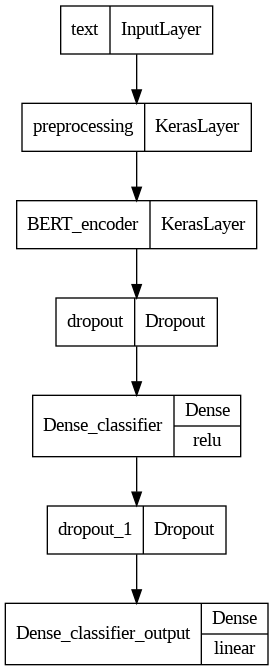
\includegraphics[scale=.55]{./p2-1}
    \caption{گراف مصور مدل}\label{fig.21}
\end{figure}

\cleardoublepage

\begin{figure}[!h]
    \centering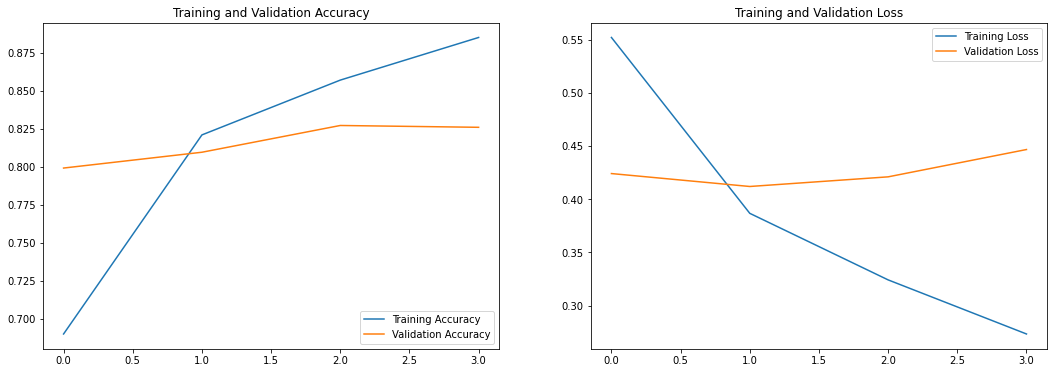
\includegraphics[scale=.45]{./p2-2}
    \caption{نمودار صحت و خطا}\label{fig.22}
\end{figure}


همانطور که مشاهده می‌شود \lr{ es-callback} باعث می‌شود که آموزش مدل به محض شروع بیش‌برازش متوقف شود. در حالتی که خطای اعتبارسنجی شروع به افزایش می‌کند، صحت آموزشی (بدون اعتبارسنجی) نزدیک 88 درصد است. درحالی که صحت اعتبارسنجی نزدیک 82 درصد است.

\cleardoublepage
% -------------------------------------------------------------------



\section{شبکه ترنسفورمر برای مسائل دیگر}
\subsection{سوال اول}


از آنجایی که بحث چت‌بات‌ها مدتی داغ است. به عنوان اولین مسئله با استفاده از این ماژول یک برنامه تولید متن نوشته شد. خروجی آن به ازای سه جمله دلخواه به همراه کد در ادامه مشاهده می‌شود.
\begin{figure}[!h]
    \centering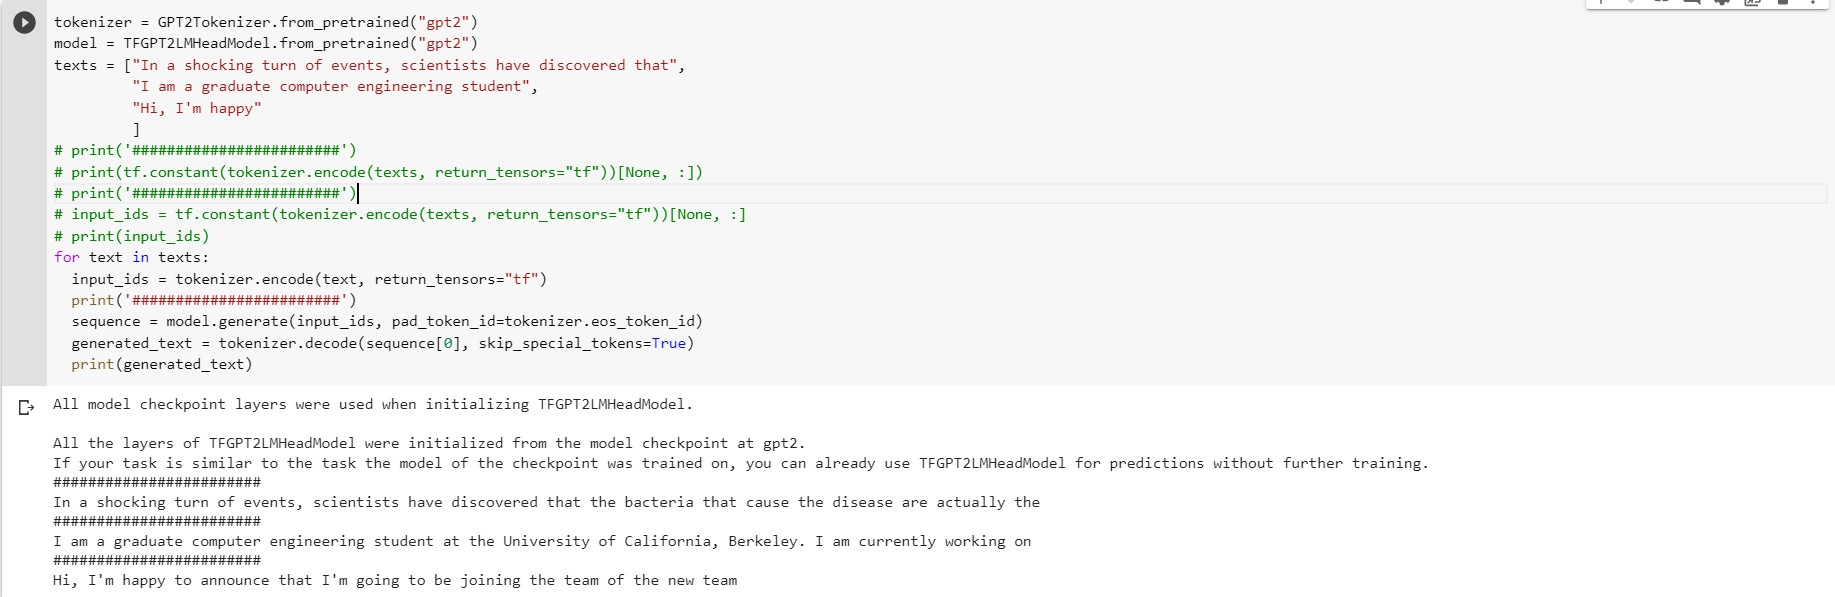
\includegraphics[scale=.40]{./p3-1}
    \caption{مدل تولید ادامه متن}\label{fig.31}
\end{figure}
\cleardoublepage

به عنوان مسئله دوم از حوزه پردازش زبان طبیعی، مسئله خلاصه‌سازی متن تست شد. خروجی آن در ادامه مشاهده می‌شود.

\begin{figure}[!h]
    \centering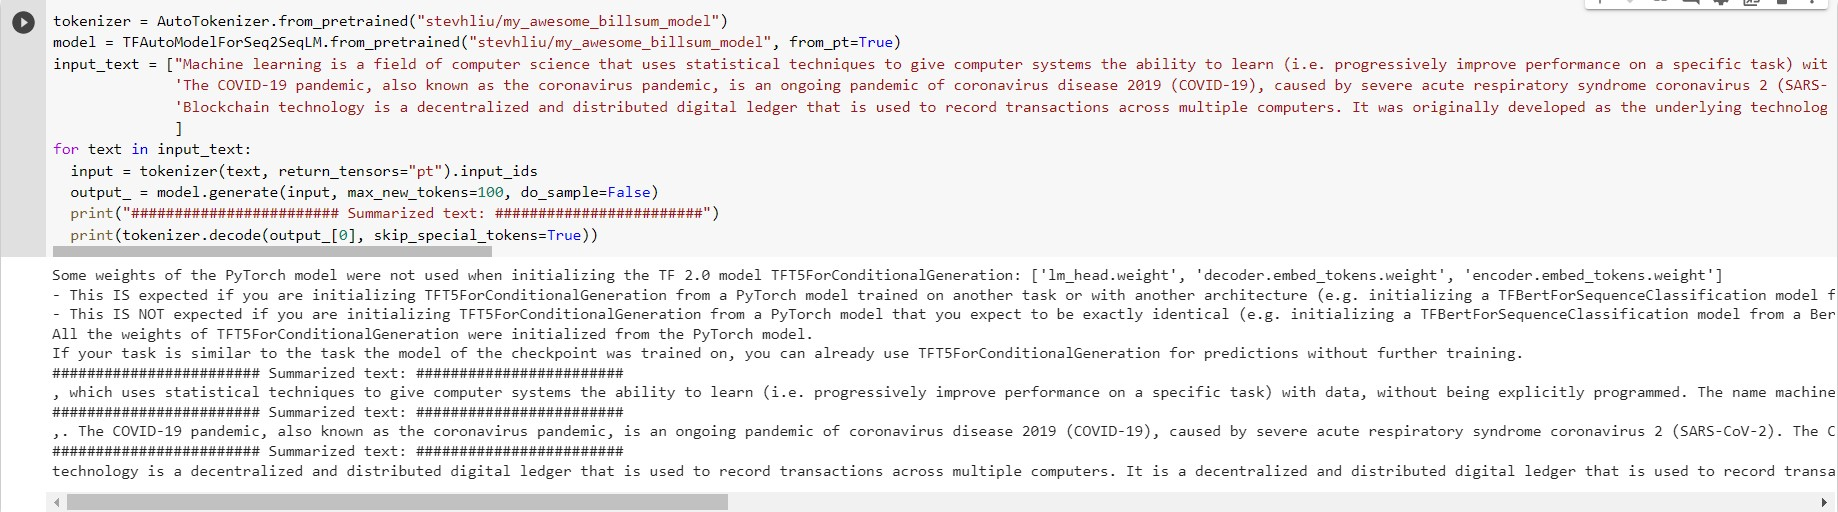
\includegraphics[scale=.40]{./p3-2}
    \caption{خلاصه‌سازی متن}\label{fig.32}
\end{figure}

\end{document}